\documentclass[border=10pt]{standalone}

\usepackage{tikz}
\usepackage{tikzsymbols}
\usetikzlibrary{calc,patterns,shapes.geometric}

\def\centerarc[#1](#2)(#3:#4:#5){\draw[#1] ($(#2)+({#5*cos(#3)},{#5*sin(#3)})$) arc (#3:#4:#5);}

\begin{document}
	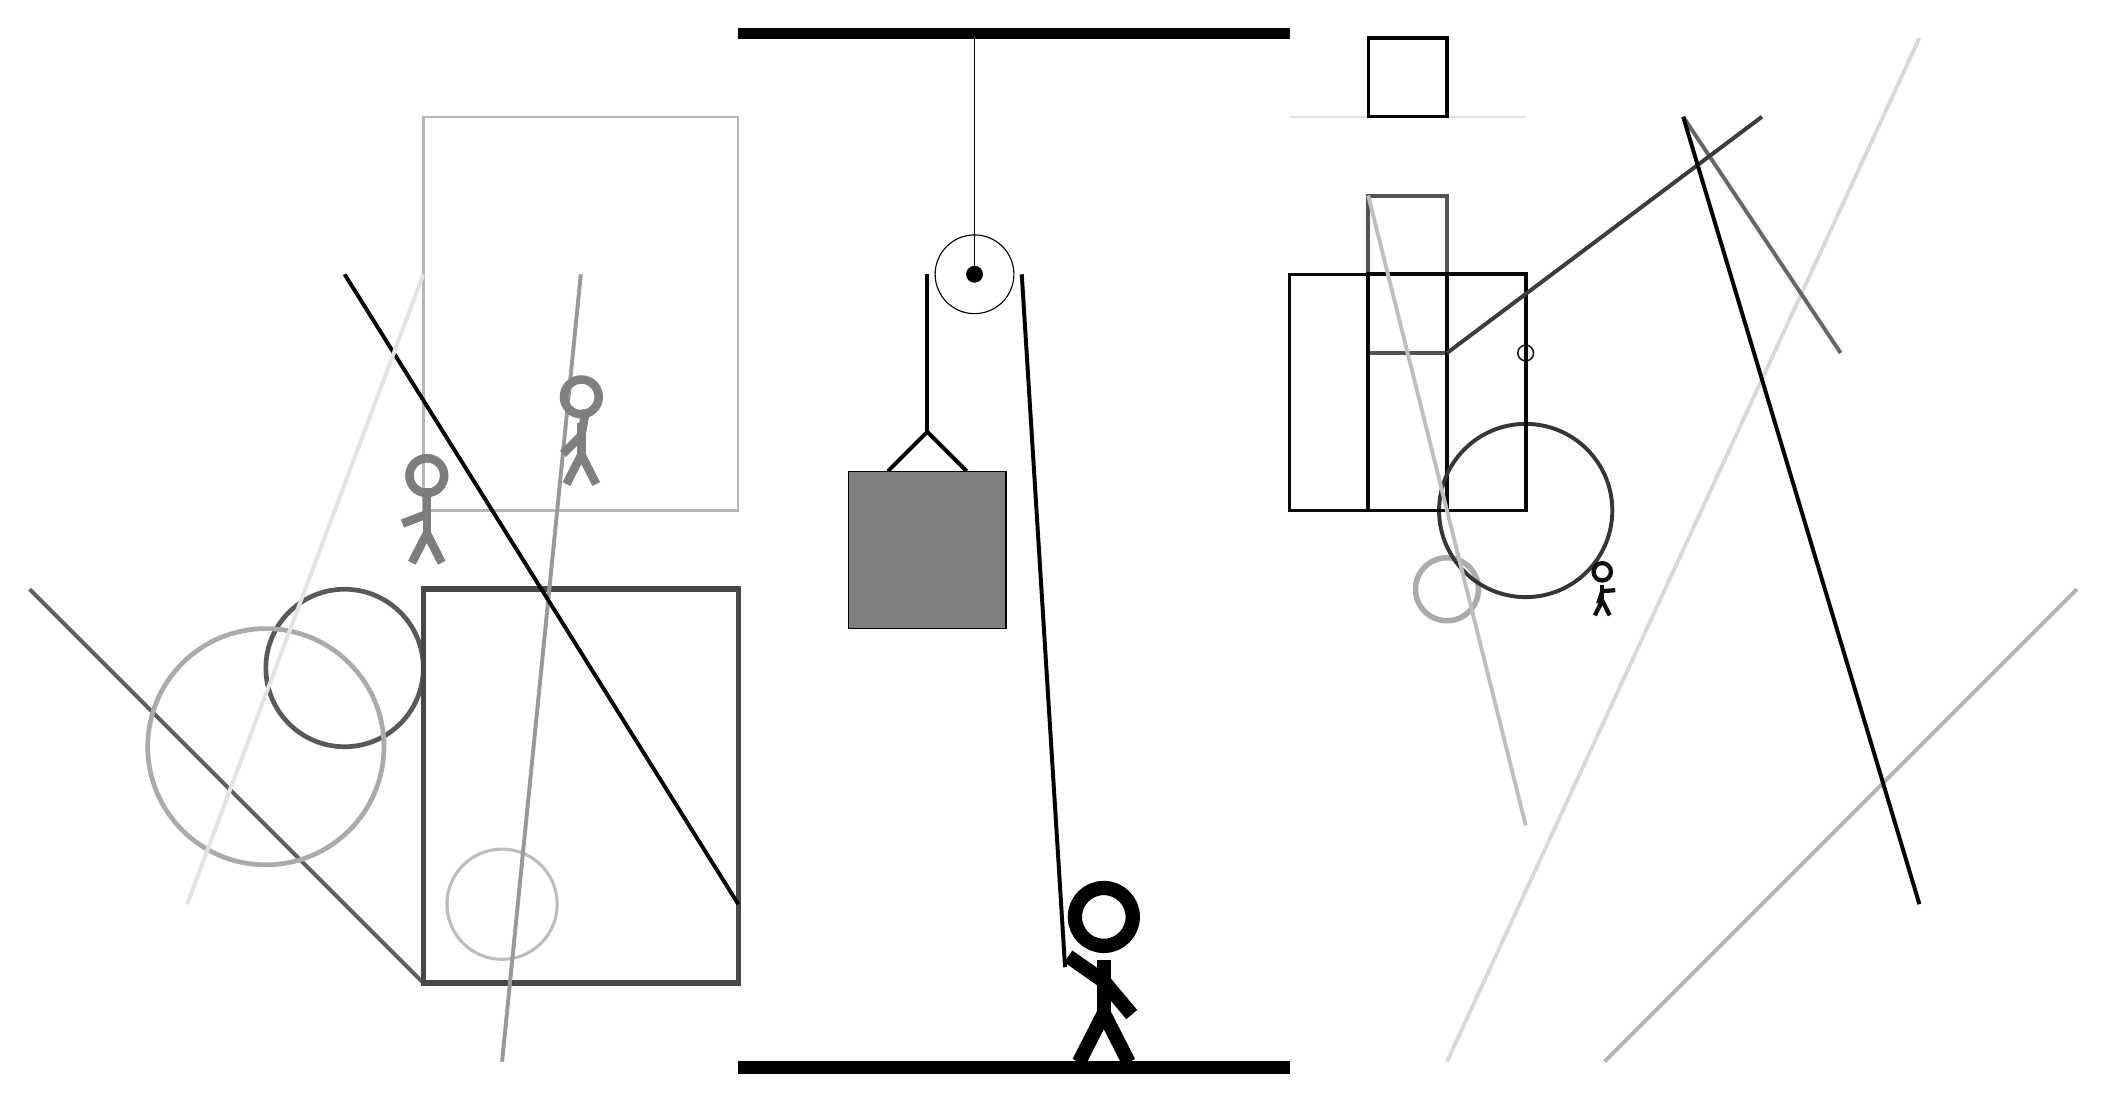
\begin{tikzpicture}
		%%%%% START %%%%%
		
		\draw[fill=black] (-2, 10) rectangle (5, 10.125);
		
		\draw (1, 7) circle (0.5);
		\draw[fill=black] (1, 7) circle (0.1);
		\draw (1, 10) -- (1, 7);
		
		\draw [line width=0.7mm, color=black!33](7, 3) circle (0.4);
		
		\draw[line width=0.5mm, color=black!67] (6, 6) rectangle (7, 8);
		\draw[line width=0.5mm, color=black!63](-6, -2) -- (-11, 3);
		\draw[line width=0.2mm, color=black!12] (5, 9) rectangle (8, 9);
		
		\draw[line width=0.4mm, color=black!96] (7, 4) rectangle (5, 7);
		
		\draw [line width=0.6mm, color=black!65](-7, 2) circle (1.0);
		
		\draw[line width=0.7mm, color=black!72] (-2, 3) rectangle (-6, -2);
		
		\draw [line width=0.5mm, color=black!79](8, 4) circle (1.1);
		\draw[line width=0.5mm, color=black!15](7, -3) -- (13, 10);
		\draw [line width=0.6mm, color=black!33](-8, 1) circle (1.5);
		\draw[line width=0.3mm, color=black!29] (-2, 9) rectangle (-6, 4);
		\node[line width=0.3mm, color=black!94] at (9, 3) {\Strichmaxerl[3][72][4]};
		\draw [line width=0.2mm, color=black!89](8, 6) circle (0.1);
		\draw [line width=0.4mm, color=black!26](-5, -1) circle (0.7);
		\draw[line width=0.5mm, color=black!97] (6, 4) rectangle (8, 7);
		\node[line width=0.5mm, color=black!51] at (-6, 4) {\Strichmaxerl[6][21][90]};
		
		\draw[line width=0.5mm, color=black!25](8, 0) -- (6, 8);
		\draw[line width=0.5mm, color=black!40](-4, 7) -- (-5, -3);
		\draw[line width=0.5mm, color=black!98](-7, 7) -- (-2, -1);
		
		\draw[line width=0.5mm, color=black!29](9, -3) -- (15, 3);
		\draw[line width=0.5mm, color=black!60](10, 9) -- (12, 6);
		
		\draw[line width=0.5mm, color=black!77](7, 6) -- (11, 9);
		
		\draw[line width=0.4mm, color=black!100] (6, 9) rectangle (7, 10);
		\node[line width=0.5mm, color=black!50] at (-4, 5) {\Strichmaxerl[6][45][80]};
		\draw[line width=0.5mm, color=black!11](-6, 7) -- (-9, -1);
		
		\draw[line width=0.5mm, color=black!99](10, 9) -- (13, -1);
		
		\draw[line width=0.5mm] (-0.1, 4.5) -- (0.4, 5.0) -- (0.9, 4.5);
		\draw[fill=black!50] (-0.6, 4.5) rectangle (1.4, 2.5);
		
		\draw[line width=0.5mm] (0.4, 7) -- (0.4, 5.0);
		\centerarc[line width=0.5mm](1, 7)(0:180:0.6);
		\draw[line width=0.5mm](1.6, 7) -- (2.15, -1.8);
		
		\node at (2.6, -1.9) {\Strichmaxerl[10][-35][-50]};
		
		\draw[fill=black] (-2, -3) rectangle (5, -3.15);
		
		%%%%% END %%%%%
	\end{tikzpicture}
\end{document}